\documentclass{standalone}
\usepackage{tikz}
\pgfdeclarelayer{background layer}
\pgfdeclarelayer{foreground layer}
\pgfsetlayers{background layer,main,foreground layer}
\begin{document}
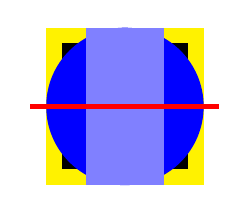
\begin{tikzpicture}
  % On main layer:
  \fill[blue] (0,0) circle [radius=1cm];
  \begin{pgfonlayer}{background layer}
    \fill[yellow] (-1,-1) rectangle (1,1);
  \end{pgfonlayer}
  \begin{pgfonlayer}{foreground layer}
    \draw[red, line width=2pt] (-1.2,0) -- (1.2,0);
  \end{pgfonlayer}
  \begin{pgfonlayer}{background layer}
    \fill[black] (-.8,-.8) rectangle (.8,.8);
  \end{pgfonlayer}
  % On main layer again:
  \fill[blue!50] (-.5,-1) rectangle (.5,1);
\end{tikzpicture}
\end{document}
